\documentclass[article]{z}
\usepackage{amsmath,bm,amssymb,dsfont}
\usepackage{multirow}
\usepackage{longtable}
%\usepackage{umlaute}
%\usepackage[utf8]{inputenc}
%\usepackage{pdfdraftcopy}
%\usepackage{/Library/Frameworks/R.framework/Resources/share/texmf/Sweave}

\DeclareMathOperator*{\argmin}{arg\,min}
\DeclareMathOperator*{\se}{se}

% To change the R input/output style:

\definecolor{Soutput}{rgb}{0,0,0.56}
\definecolor{Sinput}{rgb}{0.56,0,0}
\DefineVerbatimEnvironment{Sinput}{Verbatim}
{formatcom={\color{Sinput}},  fontsize=\footnotesize, baselinestretch=0.75}
\DefineVerbatimEnvironment{Soutput}{Verbatim}
{formatcom={\color{Soutput}}, fontsize=\footnotesize, baselinestretch=0.75}

 
%%%%%%%%%%%%%%%%%%%%%%%%%%%%%%
%% declarations for jss.cls %%%%%%%%%%%%%%%%%%%%%%%%%%%%%%%%%%%%%%%%%%
%%%%%%%%%%%%%%%%%%%%%%%%%%%%%%

%% almost as usual
\author{Robert Ferstl\\University of Regensburg \And 
        Josef Hayden\\ University of Regensburg}
\title{Zero-Coupon Yield Curve Estimation\\ with the Package \pkg{termstrc}}

%% for pretty printing and a nice hypersummary also set:
\Plainauthor{Robert Ferstl, Josef Hayden} %% comma-separated
\Plaintitle{Zero-Coupon Yield Curve Estimation with the Package termstrc} %% without formatting
\Shorttitle{Zero-Coupon Yield Curve Estimation with the Package termstrc} %% a short title (if necessary)

%% an abstract and keywords
\Abstract{
Zero-coupon yield curves and spread curves are important inputs for various financial models, e.g. pricing of securities, risk management, monetary policy issues. Since zero-coupon rates are rarely directly observable, they have to be estimated from market data. The literature broadly distinguishes between parametric and spline-based estimation methods for the zero-coupon yield curve. Our package consists of several widely-used approaches, i.e. the parametric \cite{Nelson1987} method with the \cite{Svensson1994} extension, and the \cite{McCulloch1975} cubic splines approach. Extensive summary statistics and plots are provided to compare the results of the different estimation methods. We illustrate the application of the package by practical examples using market data from European government bonds.
}
\Keywords{fixed income, term structure estimation, bond pricing, \proglang{R}}
\Plainkeywords{fixed income, term structure estimation, bond pricing, R} %% without formatting
%% at least one keyword must be supplied

%% publication information
%% NOTE: Typically, this can be left commented and will be filled out by the technical editor
%% \Volume{13}
%% \Issue{9}
%% \Month{September}
%% \Year{2004}
%% \Submitdate{2004-09-29}
%% \Acceptdate{2004-09-29}

%% The address of (at least) one author should be given
%% in the following format:
%\Address{
 % Robert Ferstl\\
 % Department of Finance\\
  %University of Regensburg\\
  %93053 Regensburg, Germany\\
 % E-mail: \email{robert.ferstl@wiwi.uni-regensburg.de}\\
 % URL: \url{http://www-finanzierung.uni-regensburg.de}\\
  
  %Josef Hayden\\
 % Department of Finance\\
 % University of Regensburg\\
  %93053 Regensburg, Germany\\
  %E-mail: \email{josef.hayden@wiwi.uni-regensburg.de}\\
 % URL: \url{http://www-finanzierung.uni-regensburg.de}
%}
%% It is also possible to add a telephone and fax number
%% before the e-mail in the following format:
%% Telephone: +43/1/31336-5053
%% Fax: +43/1/31336-734

%% for those who use Sweave please include the following line (with % symbols):
%% need no \usepackage{Sweave.sty}

%% end of declarations %%%%%%%%%%%%%%%%%%%%%%%%%%%%%%%%%%%%%%%%%%%%%%%


\begin{document}

%% include your article here, just as usual
%% Note that you should use the \pkg{}, \proglang{} and \code{} commands.
%% Note: If there is markup in \(sub)section, then it has to be escape as above.

\section{Introduction}

Hello World!
\cite{BIS2005}
\newpage
\section{Zero-coupon yield curve estimation}

\subsection{Notation}
\label{sec:notation}

Let us establish the necessary notation for a market data set of coupon bonds.

\subsubsection*{Maturity matrix}

\begin{equation}\label{maturitym}
\bm{M}_{\left[n\times m\right]}= \{m_{ij}\}
\end{equation}

The number of rows $n$ is determined through the number of cashflows of the bond $j$ with the longest maturity. For each bond $j$ exists a column with the corresponding cashflow dates. Dates after the maturity of the bond $j$ are filled up with zeros till the maturity date of the bond with the longest maturity. One element $m_{ij}$ of the matrix  refers, therefore, to the maturity date of  the $i$-th cashflow of the $j$-th bond. 

\subsubsection*{Maturity vector}

We denote with $m_j$ the maturity of the last cashflow, i.e. the maturity of the $j$-th bond.

\begin{equation}\label{weights}
    \bm{m}_{\left[1\times m\right]}= \{m_j\}
\end{equation}

\subsubsection*{Cashflow matrix}

 \begin{equation}\label{cashflowm}
\bm{C}_{\left[n\times m\right]}= \{c_{ij}\}
\end{equation}

 The cashflow matrix is defined analogously to the maturity matrix.  One element $c_{ij}$  of the matrix refers to the $i$-th cashflow of the $j$-th bond. Note, that the last cashflow of a each bond includes the redemption payment.

\subsubsection*{Discount factor matrix}

 \begin{equation}\label{discountm}
\bm{D}_{\left[n\times m\right]}= \{d_{ij}\}
\end{equation}

The discount factor matrix is also defined analogously to the maturity matrix. One element $d_{ij}$ of the matrix refers to the discount factor associated with  the $i$-th cashflow of the $j$-th bond. The discount function $d(m_{i,j})$ returns the discount factor for a given maturity. We will see in the following sections several methods how to estimate it. From an economic point of view only positve interest rates make sense. This implies that the discount factors are nonnegative where the entries in the maturity matrix are greater zero. Remember, zero entries in the maturity matrix mean that for these points in time now cash flows are associated.

\subsubsection*{Clean price vector}

 \begin{equation}\label{pc}
\bm{p}^c_{\left[1\times m\right]}= \{p^c_j\}
\end{equation}

$p_{j}^c$ is the quoted price of the $j$-th bond.

\textcolor{red}{Some blabla about price quotation on the market.}

\subsubsection*{Accrued interest vector}

  \begin{equation}\label{a}
\bm{a}_{\left[1\times m\right]}= \{a_j\}
\end{equation}


\textcolor{red}{Motivate need to calculate accrued interest. Buyer gets coupon payment but has not held bond for the whole coupon period $\dots$}

Different conventions for the calculation of accrued interest are used in the market. A basic form for the $j$-th bond is as follows.

\begin{equation}
    a_j= \frac{\mbox{number of days since last coupon payment}}{\mbox{number of days in current coupon period}}\cdot \mbox{coupon}_j
\end{equation}
 	

\subsubsection*{Dirty price vector}

The dirty price vector is the sum of the clean price vector and the accrued interest vector and consists of the dirty prices of all bonds $j$.

\begin{displaymath}
\bm{p}=\bm{p}^c+\bm{a}
\end{displaymath}

The elements are denoted by 
\begin{equation}\label{pd}
    \bm{p}_{\left[1\times m\right]}= \{p_j\}\,.
\end{equation}


\subsubsection*{Weights matrix}

In section \ref{sec:nels-svenss-meth} we will use a weighting for the estimation errors. It is constructed  as follows.

\begin{equation}\label{weights}
    \bm{\Omega}_{\left[m\times m\right]}= \begin{pmatrix}
 \omega_1 & 0 &\cdots  &0  \\
 0 & \omega_2 &  & \vdots \\
 \vdots &  & \ddots & 0 \\
 0 &\cdots  &0  & \omega_m
\end{pmatrix}
\end{equation}

Whereas $\omega_j$ is the weight for bond $j$ with duration $d_j$:

\begin{displaymath}
    \omega_j=\frac{\frac{1}{d_j}}{\sum_{i=1}^m\frac{1}{d_i}}
\end{displaymath}


The duration for a bond $j$ is a weighted average of the time to cashflows.

\textcolor{red}{Notation unclear, we would need the $j$-th column from $\bm{C,D,M}$.}

\begin{equation}\label{duration}
d_j= \frac{\bm{C}_{\left[n \times j\right]} \left(\bm{D}_{\left[n\times j\right]} \cdot \bm{M}_{\left[n\times j\right]}\right)^{\top}} {\bm{C}_{\left[n \times j\right]}\left(\bm{D}_{\left[n\times j\right]}\right)^{\top}}
\end{equation}



For the rest of the paper $(\cdot)$ denotes a element by element multiplication and $( )'$ the transposed matrix (vector). $\bm{\iota}$ denotes a column vector filled with ones.

\subsection{Indirect estimation procedure}
\label{sec:estimation}

The theoretical prices are defined as sums of the discounted cash flows of each bond.

\begin{equation}
  \label{eq:theorprices}
  \bm{\hat{p}} = \bm{\iota}'(\bm{C}\cdot\bm{D})
\end{equation}



The pricing errors
\begin{equation}
  \label{eq:pricingerrors}
  \bm{\epsilon} = \bm{p-\hat{p}}
\end{equation}

are the deviation of the theoretical prices from the dirty prices observed on the market. They satisfy

\begin{eqnarray}
  \label{eq:residuals}
  \E(\bm{\epsilon}) &=& \bm{0}\\
  \VAR(\bm{\epsilon}) &=&\sigma^2\bm{\Omega}^2 \\
  \COV(\epsilon_i, \epsilon_j) &=& 0 \quad \mbox{for}\,i\neq j\quad .
\end{eqnarray}

The goal is to minimize the weighted squared pricing errors.


\begin{equation}
  \label{eq:optimalparam}
  \hat{\bm{b}}= \argmin_{\bm{b}}\bm{\iota}'(\bm{\Omega}\bm{\epsilon}^2)
\end{equation}

Goodness of fit can be measured with the root mean squared error

\begin{equation}
  \label{eq:rmse}
  \mbox{RMSE}=\sqrt{\frac{1}{m}\bm{\iota}'(\bm{\Omega\epsilon}^2)}
\end{equation}
and the mean absolute error

\begin{equation}
  \label{eq:mae}
  \mbox{MAE}=\frac{1}{m}\bm{\iota}'|\bm{\epsilon}|\quad.
\end{equation}


%%% Local Variables: 
%%% mode: latex
%%% TeX-master: "jss-termstrc"
%%% End: 

\newpage
\section{Nelson/Siegel and Svensson method}
\label{sec:nels-svenss-meth}

\cite{Nelson1987} propose a parsimonious  model of  the instantaneous forward rate as a solution to a second-order differential equation for the case of equal roots.

\begin{equation}
  \label{eq:laguerre}
  f(m,\bm{b}) = \beta_0+\beta_1\exp\left(-\frac{m}{\tau_1}\right)+\beta_2\left[\left(\frac{m}{\tau_1}\right)\exp\left(-\frac{m}{\tau_1}\right)\right]
\end{equation}


The spot rate is the average of the instantaneous forward rates. 

\begin{equation}
  \label{eq:intspotrate}
  s(m,\bm{b})=\frac{1}{m}\int_0^mf(m,\bm{b})\,dm
\end{equation}


\begin{equation}
  \label{eq:nelson-spot}
   s(m,\bm{b}) = \beta_0 + \beta_1\frac{1-\exp(-\frac{m}{\tau_1})}{\frac{m}{\tau_1}} + \beta_2\left(\frac{1-\exp(-\frac{m}{\tau_1})}{\frac{m}{\tau_1}} - \exp(-\frac{m}{\tau_1})\right)
\end{equation}

\input{curveshape.tex}
 
\cite{Svensson1994} extension


\begin{multline}\label{eq:svensson-spot}
    s(m,\bm{b}) = \beta_0 + \beta_1\frac{1-\exp(-\frac{m}{\tau_1})}{\frac{m}{\tau_1}} + \beta_2\left(\frac{1-\exp(-\frac{m}{\tau_1})}{\frac{m}{\tau_1}} - \exp(-\frac{m}{\tau_1})\right) \\+ \beta_3\left(\frac{1-\exp(-\frac{m}{\tau_2})}{\frac{m}{\tau_2}} - \exp(-\frac{m}{\tau_2})\right)
\end{multline}



with a parameter vector ${\bm{b}} = \left(\beta_0,\beta_1,\beta_2,\tau_1,\beta_3,\tau_2\right)$.

The impact of the parameters can be described as follows \citep[see][p.7]{Bolder1999}:

\begin{itemize}
\item $\beta_0$ is the asymptotic value of the spot rate function $\lim_{m\to\infty}s(m,\bm{b})$, which can be seen as long-term interest rate.
\item $\beta_1$ is the limit of the spread between the spot rate function and the long term interest rate $\lim_{m\to\infty}\left[s(m,\bm{b})-\beta_0\right]$ determines the starting (short-term) value of the curve in terms of deviation from the asymptote (the sum $\beta_0$ and $\beta_1$) is the vertical intercept. Moreover, it defines the basic speed with which the curve tends toward its long-term trend.
\item $\beta_2$ determines the magnitude and direction of the hump. If $\beta_2 >0$  a hump will occur at  $\tau_1$, whereas $\beta_2<0$, a U-shaped value will occur at $\tau_1$.
\item $\tau_1$ is a scale parameter and specifies the position of the first hump or the U-shape on the curve ($\tau_1>0$).
\item $\beta_3$ analogously  to  $\beta_2$ determines the magnitude and direction of the second hump.
\item $\tau_2$ specifies the position of the second hump or the U-shape on the curve ($\tau_2>0$).
\end{itemize}


The discount factor for any maturity can be calculated as follows. 

\begin{displaymath}
d(m_{ij})=e^{-m_{ij}s(m_{ij},b)},
\end{displaymath}

where $s(m_{ij},b)$ is the Nelson/Siegel or Svensson spot rate function defined in \eqref{eq:nelson-spot} and \eqref{eq:svensson-spot}.

We optimize the objective function in \eqref{eq:optimalparam}. The above specification of the discount function leads to nonlinear optimization. Good starting values for the parameter vector are important to find a global minimum.



\cite{Soederlind1997} page 418 mentions that the equation for the yield has only one real root and is easy to solve numerically. They also have confidence intervals by the delta method.

This is a paramtric method \citep[see][chapter 15]{James2000}. Practioners favor smooth curve. Tradeoff with accuracy. Linear approximation is not appropriate.

\begin{itemize}
\item \cite{Geyer1999}
\item duration based weights \cite{Bliss1997}
\item derivation via Laguerre function
\item extensions \cite{Bjoerk 1999, Filipovic1999, Filipovic2000, Bjoerk2001, Bjoerk2002, Soederlind1997, Bliss1997}
\end{itemize}

%%% Local Variables: 
%%% mode: latex
%%% TeX-master: "jss-termstrc"
%%% End: 

\newpage
\section{Cubic splines}
\label{sec:cubic-splines}




%%% Local Variables: 
%%% mode: latex
%%% TeX-master: "jss-termstrc"
%%% End: 

\newpage
\section[Software implementation in R]{Software implementation in \proglang{R}}
\label{sec:soft-impl}

In this section, we describe the implementation of the package \pkg{termstrc} in the \proglang{R} system for statistical computing. The matrix-oriented notation used in sections \ref{sec:zcy-estim}-\ref{sec:cubic-splines} can efficiently be realized with base \proglang{R} functions. In the following, we give an overview about the structure of our data sets, explain the ideas behind our core functions and describe the available \proglang{S3} classes and methods provided by the package.

\subsection{Structure of data sets}

The data sets in our package have the following structure. They are \code{"list"} objects, which contain sublists for the countries available in the data set. Each of them includes market data in the format described in Table~\ref{tab:dataset}. 

\begin{table}[htb]
  \centering
  \begin{tabular}[htb]{|l|l|}
\hline
    \textbf{Object} & \textbf{Description} \\
\hline
\code{ISIN} & International Securities Identifying Number (ISIN)\\
\code{MATURITYDATE} & maturity dates\\
\code{ISSUEDATE} & issue dates\\
\code{COUPONRATE} & coupon rates as percentage of nominal values\\
\code{PRICE} & observed market prices (clean prices)\\
\code{ACCRUED} & accrued interest\\
\code{TODAY} & date when market prices were observed\\\hline
\code{CASHFLOWS\$ISIN} & International Securities Identifying Number (ISIN)\\
\code{CASHFLOWS\$CF} & all cashflows for a given ISIN\\
\code{CASHFLOWS\$DATE} & maturity dates of all cashflows\\
\hline  
\end{tabular}
  \caption{Structure of a data set}
\label{tab:dataset}
\end{table}

The first part consists of the general specifications of the bonds and its market price and accrued interest. The sublist \code{CASHFLOWS} contains all cashflows for the available bonds sorted by their ISIN and their maturity dates. This data structure is very convenient when building the cash flow matrices and the maturity matrices defined in \ref{sec:notation}.

It is easy to convert data downloaded via common data provider, e.g. \emph{Thomson Datastream}\texttrademark\, to our format.\footnote{Thomson Datastream is one of the world's largest and most respected financial statistical databases. For more information see \url{http://www.datastream.com/}.} The goal is now to perform perform zero-coupon yield curve estimations with the two procedures mentioned in Section~\ref{sec:nels-svenss-meth} and \ref{sec:cubic-splines}.

\newpage
\subsection{Core functions}
\label{sec:main-functions}

For that purpose, the package \pkg{termstrc} provides two core functions and several helper functions. \code{nelson_estim()} performs the estimation according to the parametric \cite{Nelson1987} method with the \cite{Svensson1994} extension described in Section~\ref{sec:nels-svenss-meth}.  \code{splines_estim()} allows the user to estimate the term structure according the \cite{McCulloch1975} cubic splines approach described in Section~\ref{sec:cubic-splines}. Both of the core functions require a minimum amount of input. Table~\ref{tab:corefct} gives an overview about the similar types of arguments.

\begin{table}[htb]
 \centering
 \begin{tabular}[htb]{|l|l|c|c|}
%\begin{longtable}[htb]{|l|l|c|c|}
  \hline
  \textbf{Argument}    & \textbf{Description}     & \code{nelson_estim()}       & \code{splines_estim()} \\
  \hline
\multirow{2}{1in}{\code{group}} & vector defining the group & \multirow{2}{1in}{\centering \checkmark}& \multirow{2}{1in}{\centering \checkmark}\\
                                &  of bonds used for the estimation & & \\\hline
\code{bonddata} & data set of bonds in list format & \checkmark & \checkmark \\\hline
\code{matrange} & restrict maturity range & \checkmark & \checkmark\\\hline
\multirow{2}{1in}{\code{method}} & \code{"Nelson/Siegel"} &\multirow{2}{1in}{\centering \checkmark} & \\
                                 & or \code{"Svensson"} & &\\\hline
\multirow{2}{1in}{\code{fit}} & \code{"prices"} or \code{"yields"} for&\multirow{2}{1in}{\centering \checkmark} & \\
                              & minimized squared error & &\\\hline
\multirow{2}{1in}{\code{weights}} & \code{"none"} or&\multirow{2}{1in}{\centering \checkmark} & \\
                                  & \code{"duration"} & & \\\hline
\code{startparam} & matrix of start parameters & \checkmark & \\\hline
% \vspace{1cm}\\
% \caption{Input arguments for the core functions}
% \label{tab:corefct}
% \end{longtable}
\end{tabular}
\caption{Input arguments for the core functions}
\label{tab:corefct}
 \end{table}

\subsection{Helper functions}
\label{sec:helper-functions}

Our package contains many functions to perform typical fixed income mathematics operations. Table~\ref{tab:helpfct} shows the most important ones. Most of the calculations done by the the core functions are based on the helper functions. However, the helper functions can also be applied independently. The package includes serveral more functions. For a description of them we may refer to the technical documentation. 

\begin{table}[htb]
 \centering
 \begin{tabular}[htb]{|l|l|}
\hline
\textbf{Function name} & \textbf{Description}\\\hline
\code{create_cashflows_matrix()} & creates a cashflow matrix for a group of bonds\\\hline
\code{create_maturities_matrix()} & creates a maturities matrix for a group of bonds\\\hline
\multirow{2}{1in}{\code{duration()}} & calculates Macauly duration, modified duration\\
                                 &  and duration based weights \\\hline
\multirow{2}{1in}{\code{bond\_yields()}}  & calculates yield-to-maturities with\\
                     & \code{uniroot()} function\\\hline
\code{impl_fwr()} & implied forward rates from a given spot curve\\\hline
\end{tabular}
\caption{Most important helper functions}
\label{tab:helpfct}
 \end{table}

\subsection{Exploring the estimation results}
\label{sec:expl-estim-results}

The core functions return an object of the class \code{"nelson"} or \code{"cubicsplines"}. The package offers the common
\proglang{S3} plot, print and summary methods for these classes. The objects itself is a list and contains vectors and sublists as described in Table~\ref{tab:resultsobjct}. The sublists are structured according to the chosen countries in the \code{group} argument, e.g. \code{<object>$m$<COUNTRY>} returns the maturity matrix of \code{<COUNTRY>}. 

\begin{longtable}{|l|p{4in}|c|c|}
\hline
\textbf{Object}   & \textbf{Description} & \textbf{N/S} & \textbf{CS}\\
\hline\hline
\code{group}	   & group of bonds (e.g. countries) used for the estimation & \checkmark & \checkmark\\\hline
\code{matrange}    & \code{"none"} or a vector with the maturity range& \checkmark & \checkmark\\\hline
\code{method}      & estimation method (\code{"Nelson/Siegel"} or \code{"Svensson"})& \checkmark & \\\hline
\code{fit}         & objective function (\code{"prices"}, or \code{"yields"})& \checkmark & \\\hline
\code{weights}	   & weighting of the errors used in the optimization (\code{"none"} or \code{"duration"})& \checkmark & \\\hline
\code{n_group}	   & length of object \code{group}, i.e. the number of countries& \checkmark & \checkmark\\\hline
\code{knotpoints}  & selected knot points for the cubic splines estimation & & \checkmark\\\hline
\code{spot}	   & zero-coupon yield curves as object of the class \code{"spot_curves"}& \checkmark & \checkmark\\\hline
\code{spread}	   & spread curves as object of the class \code{"s_curves"}& \checkmark & \checkmark\\\hline
\code{forward}	   & forward curves as object of the class \code{"fwr_curves"}& \checkmark & \checkmark\\\hline
\code{discount}    & discount curves as object of the class \code{"df_curves"}& \checkmark & \checkmark\\\hline
\code{expoints}    & extrapolation points for Nelson/Siegel method& \checkmark & \\\hline
\code{cf}	   & cashflow matrices& \checkmark & \checkmark\\\hline
\code{m}	   & maturity matrices& \checkmark & \checkmark\\\hline
\code{p}	   & dirty prices& \checkmark & \checkmark\\\hline
\code{phat}	   & estimated bond prices& \checkmark & \checkmark\\\hline
\code{perrors}	   & pricing errors and maturities as object of the class \code{"error"}& \checkmark & \checkmark\\\hline
\code{y}	   & bond yields& \checkmark & \checkmark\\\hline
\code{yhat}	   & estimated bond yields calculated with \code{phat}& \checkmark & \checkmark\\\hline
\code{yerrors}     & yield errors and maturities as object of the class \code{"error"}& \checkmark & \checkmark\\\hline
\code{opt_result}  & optimization results from \code{nlminb}, e.g. optimal parameters, convergence info& \checkmark & \\\hline
\code{alpha}	   & OLS coefficients of cubic splines estimation&  & \checkmark\\\hline
\code{regout}	   & OLS estimation results as object of the class \code{"lm"}&  & \checkmark\\\hline
\caption{Contents of \code{nelson} and \code{cubicsplines} object}
\label{tab:resultsobjct}
\end{longtable}

The summary methods \code{summary.nelson()} and \code{summary.cubicsplines()} give goodness of fit measures, i.e. the RMSE and MAE for the pricing and yield errors. \code{summary.nelson()} additionally shows convergence information from the solver \code{nlminb()}.

The parameters for the cubic splines approach are estimated with OLS by using the \code{lm()} function. Therefore, \code{summary.cubicsplines()} also provides summary statistics for the OLS estimation by applying \code{summary.lm(<object>$regout)}. 

The print methods \code{print.nelson()} and \code{print.cubicsplines()} return the estimated parameters in a clearly arranged way.
As Table~\ref{tab:resultsobjct} shows, the returned object from our estimation itself contains objects of certain classes. For objects of the class \code{"spot_curves", "fwr_curves", "df_curves"} and \code{"error"} plot methods are available. They will be covered in the following section. For the sublists in \code{regout}, which are objects of the class \code{"lm"}, the standard methods for the \code{"lm"} class apply.  

\newpage
\subsection{Visualization of the results}
\label{sec:visu-results}

The \proglang{S3} plot methods \code{plot.nelson()} and \code{plot.cubicsplines()} offer the following possibilities:

\begin{itemize}
\item plot zero-coupon, forward, discount or spread curves
\item return single/multiple plots for the estimated group of bonds
\item show error plots for pricing/yield errors to identify outliers
\end{itemize}

Plots of the zero-coupon yield curve for a single country include additional information. In detail, 
also the yield-to-maturities are plotted and for objects of the class \code{"cubicsplines"} the knot points used for the estimationand the 95\% confidence intervall of the zero-coupon yield curve is plotted. 

Both plot methods depend on plot methods for the classes \code{"spot\_curves", "fwr\_curves"} and \code{"df\_curves"}. These plot methods are itself based on the plot method for the class \code{"ir\_curve"}, which is the most granular class.
A object of the class \code{"spot\_curves", "fwr\_curves"} or \code{"df\_curves"} can therefore consist of serveral 
objects of the class \code{"ir\_curve"}. The advantage for the user is, that when he
is exploring a \code{"nelson"} or \code{"cubicsplines"} object, he can plot the different curves at every hierarchical level of the object. For example, the command \code{plot(<object>$spot$<COUNTRY>)} creates a plot of the spot curve of \code{<COUNTRY>}, while \code{plot(<object>$spot)} plots the spot curves of all countries. 


\subsection{Perfomance issues}
\label{sec:perfomance-issues}

The implementation of the \pkg{termstrc} package is based on an efficent operation on the data sets in list format. We avoid programming loops by using apply-functions. The most time-consuming tasks are solving the nonlinear optimization problem for the \cite{Nelson1987} and \cite{Svensson1994} method and the ordinary least squares estimation of the \cite{McCulloch1975} cubic splines. In Section~\ref{sec:rolling-estim}, we will see results for a rolling estimation procedure performed on a large data set.

%%% Local Variables: 
%%% mode: latex
%%% TeX-master: "jss-termstrc"
%%% End: 


\section{Practical application}
\label{sec:pract-appl}

The goverment debt market is the common data source for estimating a zero-coupon yield curve of a country. Government bonds are usually the most liquid securities, and can be considered default-free, provided the issuing country has a good rating. We demonstrate the application of our package with a data set of European government bonds obtained from Thomson Financial Datastream. The following examples show the application of the package using the before mentioned procedures, as well as a rolling estimation of the zero-coupon yield curve.


\subsection{Nelson/Siegel}

\begin{Schunk}
\begin{Sinput}
> library(termstrc)
\end{Sinput}
\end{Schunk}

\begin{Schunk}
\begin{Sinput}
> data(eurobonds)
> group <- c("GERMANY", "AUSTRIA", "ITALY")
> bonddata <- eurobonds
> matrange <- c(2, 12)
> method <- "Nelson/Siegel"
> fit <- "prices"
> weights <- "none"
> control <- list(eval.max = 1e+05)
> b <- matrix(c(0, 0, 0, 1, 0, 0, 0, 1, 0, 0, 0, 1), nrow = 3, 
+     ncol = 4, byrow = TRUE)
> rownames(b) <- group
> colnames(b) <- c("beta0", "beta1", "beta2", "tau1")
\end{Sinput}
\end{Schunk}

\begin{Schunk}
\begin{Sinput}
> x <- nelson_estim(group, bonddata, matrange, method, fit, weights, 
+     startparam = b, control)
> print(x)
\end{Sinput}
\begin{Soutput}
---------------------------------------------------
Parameters for Nelson/Siegel, Svensson estimation:

Method: Nelson/Siegel 
Fitted: prices 
Weights: none 

---------------------------------------------------

             GERMANY     AUSTRIA       ITALY
beta_0  0.0418991850  0.04167176  0.04645068
beta_1 -0.0190504299 -0.01716246 -0.02012130
beta_2 -0.0001155352 -0.01451567 -0.02134967
tau_1   3.9893303512  2.11920557  2.39845119

---------------------------------------------------
Parameters for Nelson/Siegel, Svensson estimation:

Method: Nelson/Siegel 
Fitted: prices 
Weights: none 

---------------------------------------------------

             GERMANY     AUSTRIA       ITALY
beta_0  0.0418991850  0.04167176  0.04645068
beta_1 -0.0190504299 -0.01716246 -0.02012130
beta_2 -0.0001155352 -0.01451567 -0.02134967
tau_1   3.9893303512  2.11920557  2.39845119
\end{Soutput}
\end{Schunk}

\begin{Schunk}
\begin{Sinput}
> summary(x)
\end{Sinput}
\begin{Soutput}
---------------------------------------------------
Goodness of fit:
---------------------------------------------------

                  GERMANY      AUSTRIA        ITALY
RMSE-Prices  1.059285e-01 2.868050e-02 0.0790745094
AABSE-Prices 6.157349e-02 2.000662e-02 0.0561561019
RMSE-Yields  1.324394e-04 4.051508e-05 0.0001240929
AABSE-Yields 8.941224e-05 2.994120e-05 0.0001016403


---------------------------------------------------
Convergence information:
---------------------------------------------------

        Convergence ()  
GERMANY "no convergence"
AUSTRIA "converged"     
ITALY   "converged"     

        Solver message                                   
GERMANY "iteration limit reached without convergence (9)"
AUSTRIA "relative convergence (4)"                       
ITALY   "relative convergence (4)"                       
\end{Soutput}
\end{Schunk}

\begin{center}
\begin{Schunk}
\begin{Sinput}
> par(mfrow = c(3, 2), cex = 0.55)
> plot(x)
\end{Sinput}
\end{Schunk}
\includegraphics{example-005}
\end{center}

\subsection{Cubic Splines}

\begin{Schunk}
\begin{Sinput}
> data(eurobonds)
> group <- c("GERMANY", "AUSTRIA", "ITALY")
> bonddata <- eurobonds
> matrange <- "all"
\end{Sinput}
\end{Schunk}

\begin{Schunk}
\begin{Sinput}
> x <- splines_estim(group, bonddata, matrange)
> print(x)
\end{Sinput}
\begin{Soutput}
---------------------------------------------------
Parameters for Cubic splines estimation:

[1] "GERMANY:"
      alpha 1       alpha 2       alpha 3       alpha 4       alpha 5 
-0.0031562638 -0.0001804021  0.0008893256  0.0009869789 -0.0235685086 

[1] "AUSTRIA:"
      alpha 1       alpha 2       alpha 3       alpha 4 
-0.0030226383  0.0007101622  0.0010939255 -0.0234513152 

[1] "ITALY:"
      alpha 1       alpha 2       alpha 3       alpha 4       alpha 5 
-1.319834e-03 -2.612472e-03 -3.871354e-05  1.264864e-03  6.204093e-04 
      alpha 6 
-2.481481e-02 
\end{Soutput}
\end{Schunk}


\begin{Schunk}
\begin{Sinput}
> summary(x)
\end{Sinput}
\begin{Soutput}
---------------------------------------------------
Goodness of fit:
---------------------------------------------------

                  GERMANY      AUSTRIA        ITALY
RMSE-Prices  1.818950e+01 1.386148e+01 2.283539e+01
AABSE-Prices 1.406844e+01 8.328159e+00 1.536100e+01
RMSE-Yields  1.224657e-04 1.114989e-04 1.499874e-04
AABSE-Yields 8.282076e-05 8.727466e-05 1.155357e-04

---------------------------------------------------
Summary statistics for the fitted models:
---------------------------------------------------

$GERMANY

Call:
lm(formula = -Y[[k]] ~ X[[k]] - 1)

Residuals:
      Min        1Q    Median        3Q       Max 
-0.133728 -0.043399 -0.009263  0.019054  0.337135 

Coefficients:
          Estimate Std. Error t value Pr(>|t|)    
alpha 1 -3.156e-03  4.765e-04  -6.623 7.51e-07 ***
alpha 2 -1.804e-04  1.572e-04  -1.148    0.262    
alpha 3  8.893e-04  4.782e-05  18.598 9.25e-16 ***
alpha 4  9.870e-04  6.148e-05  16.053 2.45e-14 ***
alpha 5 -2.357e-02  5.786e-04 -40.734  < 2e-16 ***
---
Signif. codes:  0 ‘***’ 0.001 ‘**’ 0.01 ‘*’ 0.05 ‘.’ 0.1 ‘ ’ 1 

Residual standard error: 0.1084 on 24 degrees of freedom
Multiple R-Squared:     1,	Adjusted R-squared:     1 
F-statistic: 1.693e+06 on 5 and 24 DF,  p-value: < 2.2e-16 


$AUSTRIA

Call:
lm(formula = -Y[[k]] ~ X[[k]] - 1)

Residuals:
       Min         1Q     Median         3Q        Max 
-0.0806338 -0.0430618  0.0006852  0.0263651  0.1077566 

Coefficients:
          Estimate Std. Error t value Pr(>|t|)    
alpha 1 -3.023e-03  1.274e-04  -23.72 4.03e-10 ***
alpha 2  7.102e-04  4.795e-05   14.81 3.95e-08 ***
alpha 3  1.094e-03  8.459e-05   12.93 1.44e-07 ***
alpha 4 -2.345e-02  2.255e-04 -104.01  < 2e-16 ***
---
Signif. codes:  0 ‘***’ 0.001 ‘**’ 0.01 ‘*’ 0.05 ‘.’ 0.1 ‘ ’ 1 

Residual standard error: 0.05827 on 10 degrees of freedom
Multiple R-Squared:     1,	Adjusted R-squared:     1 
F-statistic: 1.479e+06 on 4 and 10 DF,  p-value: < 2.2e-16 


$ITALY

Call:
lm(formula = -Y[[k]] ~ X[[k]] - 1)

Residuals:
      Min        1Q    Median        3Q       Max 
-0.268791 -0.051542 -0.003029  0.056274  0.162438 

Coefficients:
          Estimate Std. Error t value Pr(>|t|)    
alpha 1 -1.320e-03  1.827e-03  -0.722    0.476    
alpha 2 -2.612e-03  4.548e-04  -5.745 2.85e-06 ***
alpha 3 -3.871e-05  9.279e-05  -0.417    0.679    
alpha 4  1.265e-03  4.061e-05  31.149  < 2e-16 ***
alpha 5  6.204e-04  6.910e-05   8.978 5.29e-10 ***
alpha 6 -2.481e-02  1.180e-03 -21.029  < 2e-16 ***
---
Signif. codes:  0 ‘***’ 0.001 ‘**’ 0.01 ‘*’ 0.05 ‘.’ 0.1 ‘ ’ 1 

Residual standard error: 0.1005 on 30 degrees of freedom
Multiple R-Squared:     1,	Adjusted R-squared:     1 
F-statistic: 2.049e+06 on 6 and 30 DF,  p-value: < 2.2e-16 
\end{Soutput}
\end{Schunk}

\begin{center}
\begin{Schunk}
\begin{Sinput}
> par(mfrow = c(3, 2), cex = 0.55)
> plot(x)
\end{Sinput}
\end{Schunk}
\includegraphics{example-009}
\end{center}




%\clearpage
\subsection{Rolling estimation procedure}

We now provide results of a daily rolling estimation of the zero-coupon yield curve for the time between November 30, 2007 and February 1, 2008. We use the \cite{Svensson1994} method, together with duration weights and minimization of the price errors. Figure \ref{fig:3dplot} shows the estimated French yield curves during that time period.

\begin{figure}[htb]
  \begin{center}
  \caption{Zero-coupon yield curves in France}
  \label{fig:3dplot}
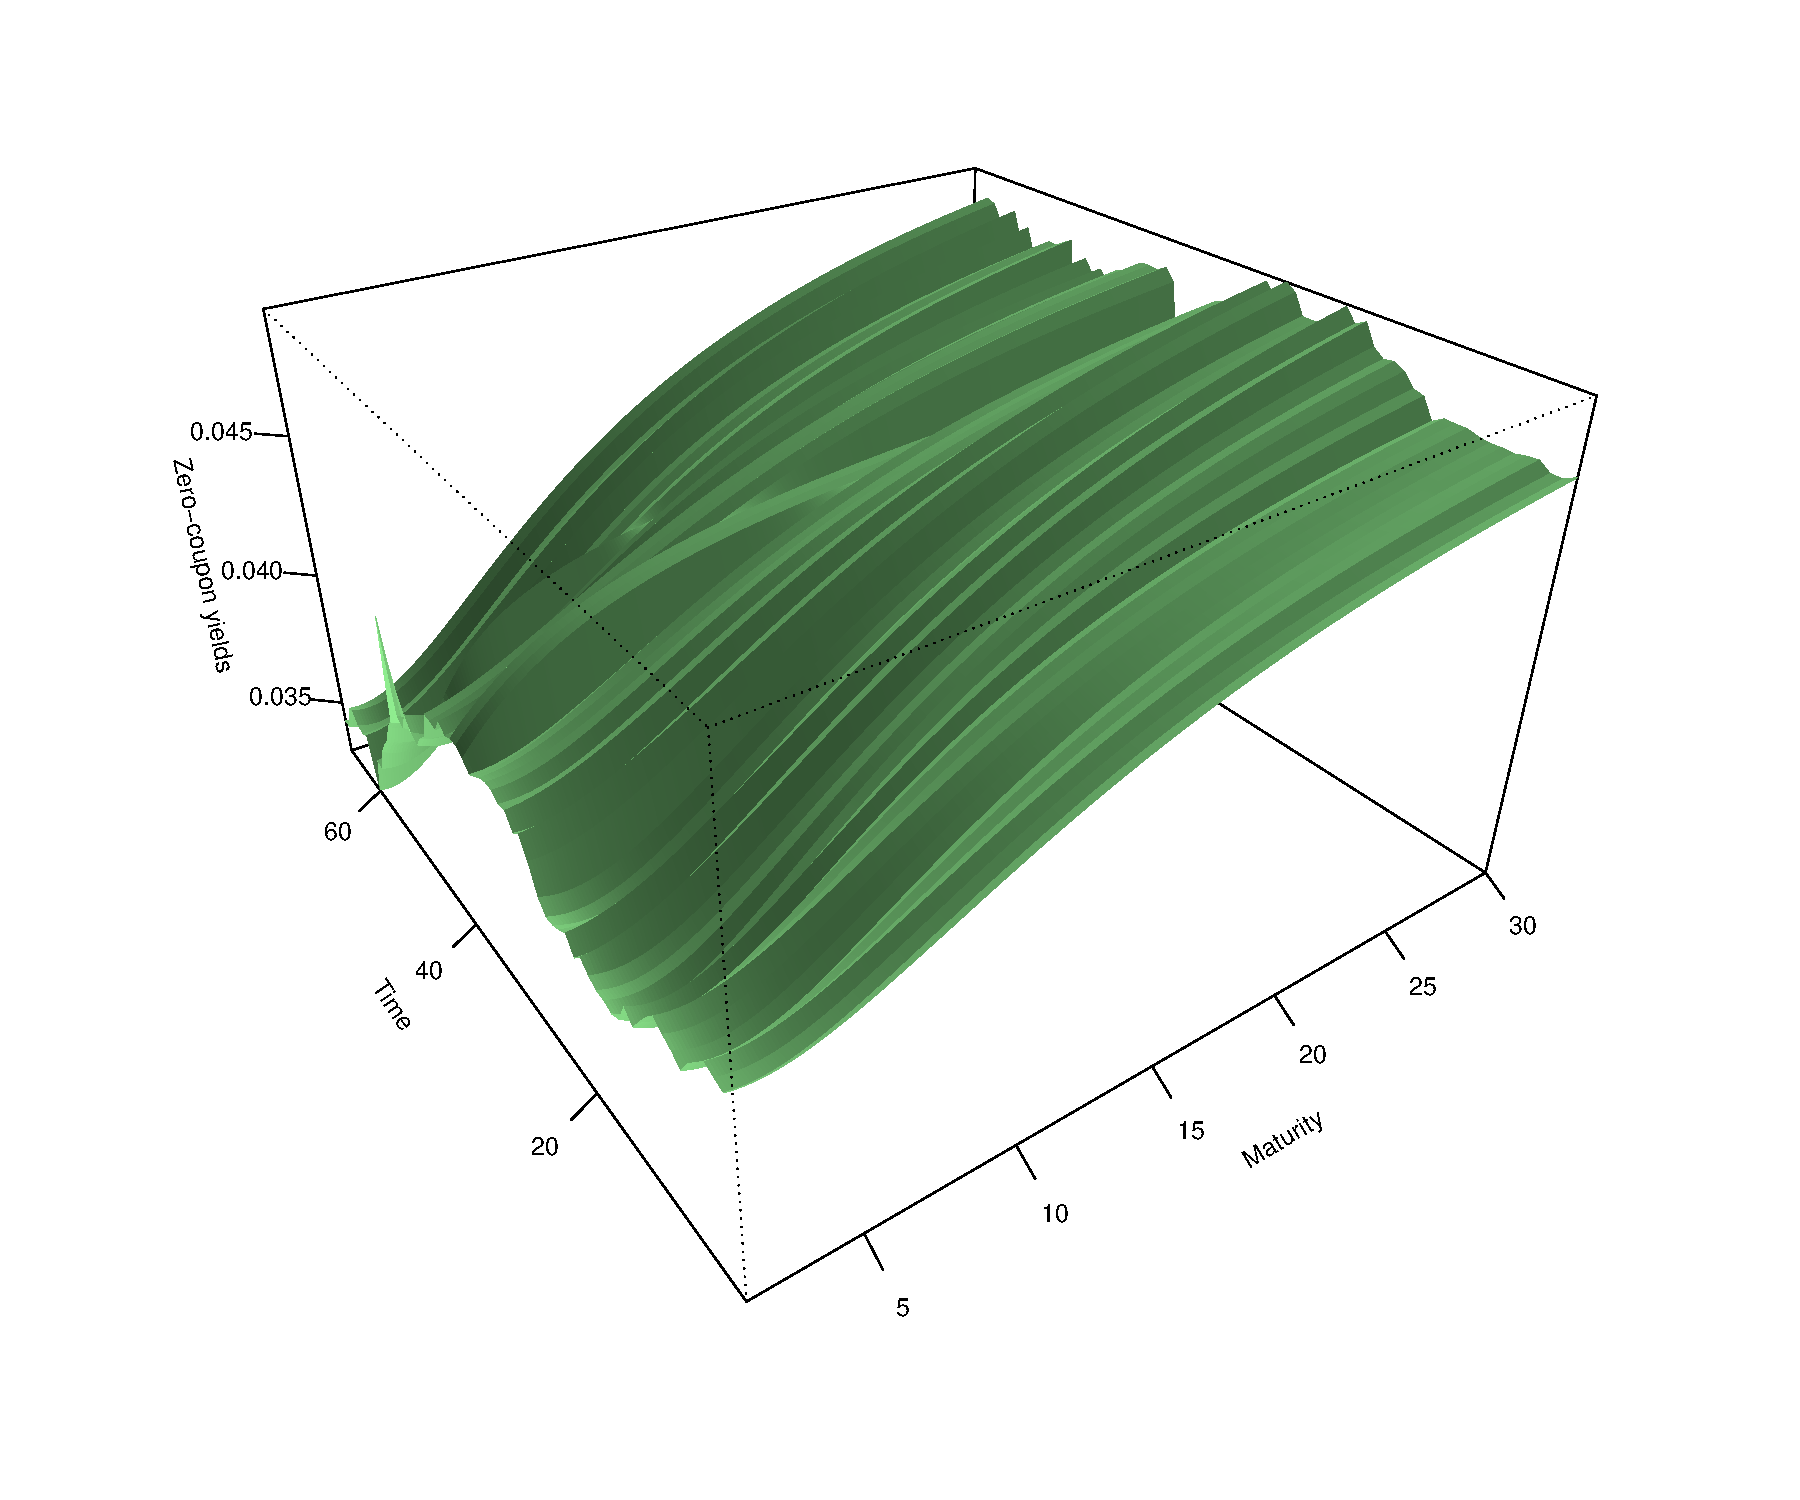
\includegraphics[width=0.7\textwidth]{3dplot}
\end{center}
\end{figure}

The estimated parameters are presented in Figure \ref{fig:paramdevel}. To speed up the estimation and ensure that the algorithm stays in a global minimum, the estimated parameters from the previous period were used as starting values for the next one.

\begin{figure}[htb]
  \begin{center}
  \caption{Estimated parameters}
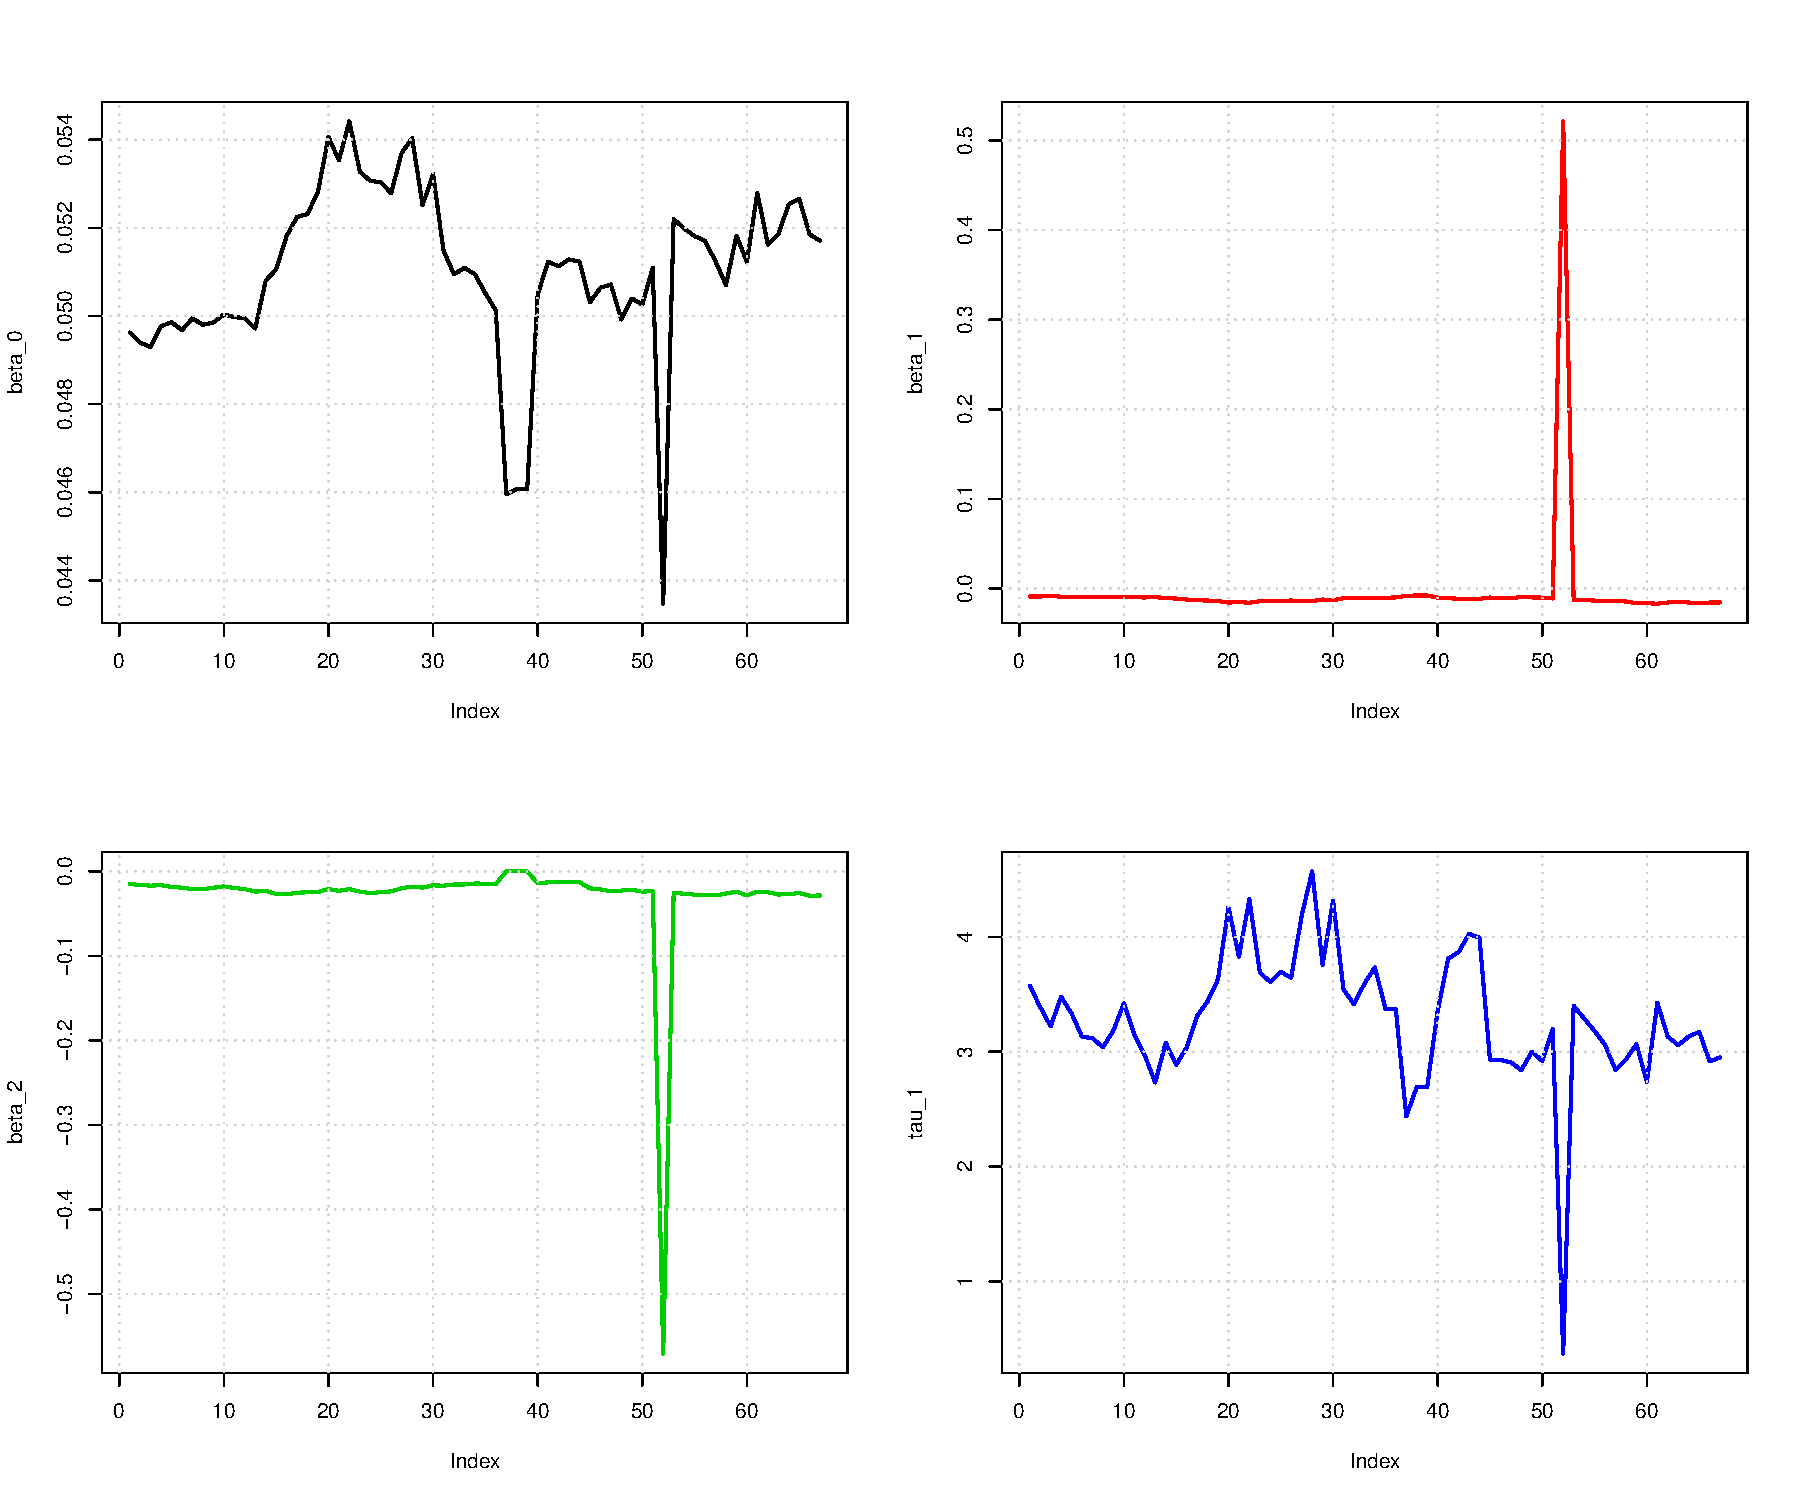
\includegraphics[width=0.8\textwidth]{paramdevel}
\label{fig:paramdevel}
\end{center}
\end{figure}



%%% Local Variables: 
%%% mode: latex
%%% TeX-master: "jss-termstrc"
%%% End: 
%\clearpage
\section{Discussion}

\begin{itemize}
\item extensions for credit spread estimation \cite{Jankowitsch2004, Geyer2004}
\item extensions for splines: exponential splines by \cite{Vasicek1982} (leads to more realisitc shapes of the forward curve), \cite{Adams1994} obtain maximum smoothness, \cite{Fisher1995, Waggoner1997, Anderson1999 }
\end{itemize}
\clearpage
\section{Conclusion}
\label{sec:conclusion}

In this paper, we presented the \proglang{R} extension package \pkg{termstrc}. It provides functions for the estimation of zero-coupon yield curves from market data of coupon bonds. The package covers the two most widely-used approaches in practice and provides a simple interface to them. The results contain detailed summaries about the estimation, as well as graphical outputs of spot, forward and credit spread curves.


\section*{Acknowledgments}

The authors want to thank Alois Geyer and Kurt Hornik for their comments about the package and the paper.


%%% Local Variables: 
%%% mode: latex
%%% TeX-master: "jss-termstrc"
%%% End: 

%\clearpage

%\nocite{*}
%\listoftables
%\listoffigures
\bibliographystyle{jss}
\bibliography{termstrc}

\end{document}


%%% Local Variables: 
%%% mode: latex
%%% TeX-master: t
%%% End: 
